\documentclass{article}

\usepackage{booktabs}
\usepackage{tabularx}
\usepackage{color}
\usepackage[colorlinks,linkcolor=blue]{hyperref}
\usepackage{graphicx}

\title{SE 3XA3: Development Plan\\Garden Defender}

\author{Team 29
		\\ Ashley Williams, willia18
		\\ Declan Mullane, mullanem
		\\ Leo Shi, shiy12
}

\date{}

%\input{../Comments}

\begin{document}

\begin{table}[hp]
\caption{Revision History} \label{TblRevisionHistory}
\begin{tabularx}{\textwidth}{llX}
\toprule
\textbf{Date} & \textbf{Developer(s)} & \textbf{Change}\\
\midrule
Sept. 25 & Ashley Williams & Initial Draft\\
Sept. 25 & Declan Mullane & Initial Draft\\
Sept. 25 & Leo Shi & Initial Draft\\
Sept. 28 & Ashley Williams & Revision 0\\
Sept. 28 & Declan Mullane & Revision 0\\
Sept. 28 & Leo Shi & Revision 0\\
\bottomrule
\end{tabularx}
\end{table}

\newpage

\maketitle

\section{Team Meeting Plan}
Team meetings will be held three times every week and require attendance by all members. Aside from the two meetings during lab time, our third meeting will take place at Mills Memorial Library on Friday afternoon. Our meetings will generally focus on upcoming milestones and ensuring that every process is on track. We will alternate the role of scribe weekly.  The scribe/chair is responsible for the preparation of topics before meetings and ensuring that meetings run smoothly. The meeting agenda shown below will be used to record essential information, like decisions made during each meeting.(credit from \href{https://officetemplatesonline.com/download/download-formal-meeting-agenda-template/}{\textcolor{blue} {OfficeTemplateOnline.com}} )


\begin{figure}[htbp]
\centering
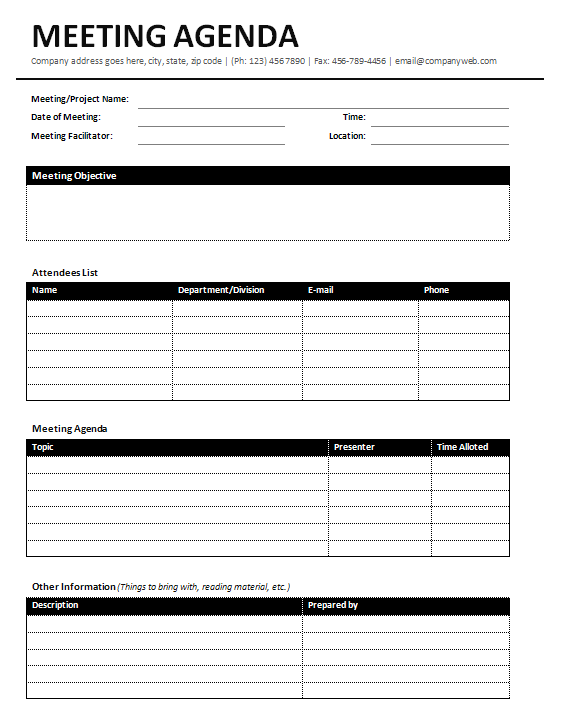
\includegraphics[scale=0.7]{MeetingAgenda.png}
\caption{MeetingAgenda}
\end{figure}


\newpage
\section{Team Communication Plan}
The primary means of communication will be Facebook, to coordinate meetings, discuss any other small issues, or make clarifications.  We will use Git to track more technical aspects of the project. 

\section{Team Member Roles}
There will be no team leader; we are all equally responsible and accountable.  The scribe/chair will alternate weekly.

\section{Git Workflow Plan}
 Most of our documentation will be done and released using the Master branch. All milestones and major revisions will be labelled and tagged on this branch. We will make use of the feature branch in order to create an isolated environment for both developing and testing, specifically when members are responsible for writing different sections of code.

\section{Proof of Concept Demonstration Plan}

For our demonstration, we want to show that the basic requirements of our game have been met, or are well on their way to being achieved. It is important that player and enemy characters are displayed properly in the GUI, and that other in-game actions work as expected.  For instance, attacks made by the player character must register properly - if a projectile hits the enemy, its avatar should no longer appear on screen. Likewise, a projectile that misses the enemy shouldn't remove its avatar. Ensuring that our game is functional is our main objective for our proof of concept; other aspects of our game, such as graphics, are secondary goals.


\section{Technology}
The following technologies will be used in this project:
\begin{itemize}

  \item HTML - Standard markup language for creating web pages
  \item CSS -  Style sheet language for styling web pages
  \item JavaScript - Interpreted programming language for web page applications
  \item pixi.js - JavaScript game engine
  \item Jasmine - JavaScript Unit Testing Framework
  \item WebStorm - JavaScript IDE
  \item JSDoc - JavaScript documentation generator

\end{itemize}


\section{Coding Style}
 We will follow the standard indicated at \href{https://standardjs.com/}{\textcolor{blue} {JavaScript Standard Style}}

\section{Project Schedule}

Project schedule can be found at  \href{https://gitlab.cas.mcmaster.ca/shiy12/3XA3Group29/tree/master/Game1/ProjectSchedule}{\textcolor{blue} {Garden Defender Project Schedule}}

\section{Project Review}

\end{document}